\documentclass[11pt,a4paper]{article}
\usepackage[utf8]{inputenc}
\usepackage[T1]{fontenc}
\usepackage{tgpagella}
\usepackage[spanish]{babel}
\usepackage{geometry}
\usepackage{booktabs}
\usepackage{xcolor}
\usepackage{titlesec}
\usepackage{fancyhdr}
\usepackage[parfill]{parskip}
\usepackage[expansion=false]{microtype}
\usepackage{hyperref}
\usepackage{setspace}
\usepackage{graphicx}
\usepackage{needspace}

\widowpenalty=10000
\clubpenalty=10000
\displaywidowpenalty=10000

\geometry{top=3.0cm,bottom=3.0cm,left=3.5cm,right=3.5cm}
\setlength{\parskip}{0.65em}
\setlength{\parindent}{0em}

\definecolor{azulai}{RGB}{30,80,140}
\definecolor{doradoai}{RGB}{140,90,0}
\definecolor{grisai}{RGB}{70,70,70}

\titleformat{\section}{\Large\bfseries\color{azulai}}{}{0em}{}[{\color{azulai}\titlerule[0.5pt]}]
\titlespacing*{\section}{0pt}{1.4em}{0.5em}

\titleformat{\subsection}{\large\bfseries\color{doradoai}}{}{0em}{}
\titlespacing*{\subsection}{0pt}{1.0em}{0.35em}

\titleformat{\subsubsection}{\normalsize\bfseries\color{grisai}}{}{0em}{}
\titlespacing*{\subsubsection}{0pt}{0.7em}{0.25em}

\pagestyle{fancy}\fancyhf{}
\rhead{\textcolor{grisai}{\small Izas — Arquitectura Interna}}
\lhead{\textcolor{grisai}{\small Plutón · Casa 8 · Casa 12 · Quirón · Lilith}}
\cfoot{\textcolor{grisai}{\small\thepage}}
\renewcommand{\headrulewidth}{0.3pt}

\hypersetup{colorlinks=true,linkcolor=azulai,urlcolor=azulai}
\setstretch{1.25}
\tolerance=1500
\emergencystretch=4em

\begin{document}

\begin{titlepage}
  \centering
  \vspace*{1.5cm}
  {\Huge\bfseries\color{azulai} Plutón · Casa 8 · Casa 12}\\[0.35cm]
  {\Huge\bfseries\color{azulai} Quirón · Lilith}\\[0.5cm]
  {\large\color{grisai} Arquitectura Interna}\\[0.3cm]
  {\small\itshape\color{grisai} Sombra, herida, intimidad y profundidad psíquica}\\[2cm]
  {\huge\color{doradoai} Izas}\\[1.5cm]
  {\Large 16/04/1979 \quad 04:20}\\[0.3cm]
  {\Large Pamplona, España}\\[0.3cm]
  {\normalsize Lat: 42.8157° \quad Lon: -1.6522° \quad UTC+02:00}\\[0.3cm]
  {\normalsize Ascendente: Acuario 6°20' \quad
    MC: Escorpio 29°12'}\\[2cm]

  \begin{tabular}{ll}
    \textbf{Plutón:}  & Libra — Casa 8 17°38' (retrógrado) \\
    \textbf{Quirón:}  & Tauro — Casa 3 8°29' \\
    \textbf{Lilith:}  & Leo — Casa 7 20°38' \\
    \textbf{Casa 8:}  & Virgo \\
    \textbf{Casa 12:} & Capricornio \\
  \end{tabular}\\[2cm]

  \vfill
  {\small Generado el 20/05/2026}
\end{titlepage}

\tableofcontents
\newpage

\section{Datos de referencia}

\begin{center}
\begin{tabular}{llll}
  \toprule
  \textbf{Punto} & \textbf{Signo} & \textbf{Casa} & \textbf{Posición} \\
  \midrule
  Plutón (retrógrado) & Libra & 8 & 17°38' \\
  Quirón & Tauro & 3 & 8°29' \\
  Lilith          & Leo & 7 & 20°38' \\
  Casa 8          & Virgo             & ---                  & --- \\
  Casa 12         & Capricornio            & ---                  & --- \\
  Ascendente      & Acuario         & ---                  & 6°20' \\
  Medio Cielo     & Escorpio          & ---                  & 29°12' \\
  \bottomrule
\end{tabular}
\end{center}

\vspace{0.5cm}
\textbf{Aspectos relevantes:}

\begin{center}
\begin{tabular}{lllll}
  \toprule
  \textbf{Punto 1} & \textbf{Asp.} & \textbf{Punto 2} & \textbf{Aspecto} & \textbf{Orbe} \\
  \midrule
  Plutón & sex & Neptuno & Sextil & 2.7° \\
  Plutón & opo & Sol & Oposición & 7.9° \\
  Quirón & tri & Saturno & Trígono & 0.9° \\
  Lilith & tri & Neptuno & Trígono & 0.3° \\
  Lilith & cua & Urano & Cuadratura & 0.7° \\
  \bottomrule
\end{tabular}
\end{center}

\begin{center}
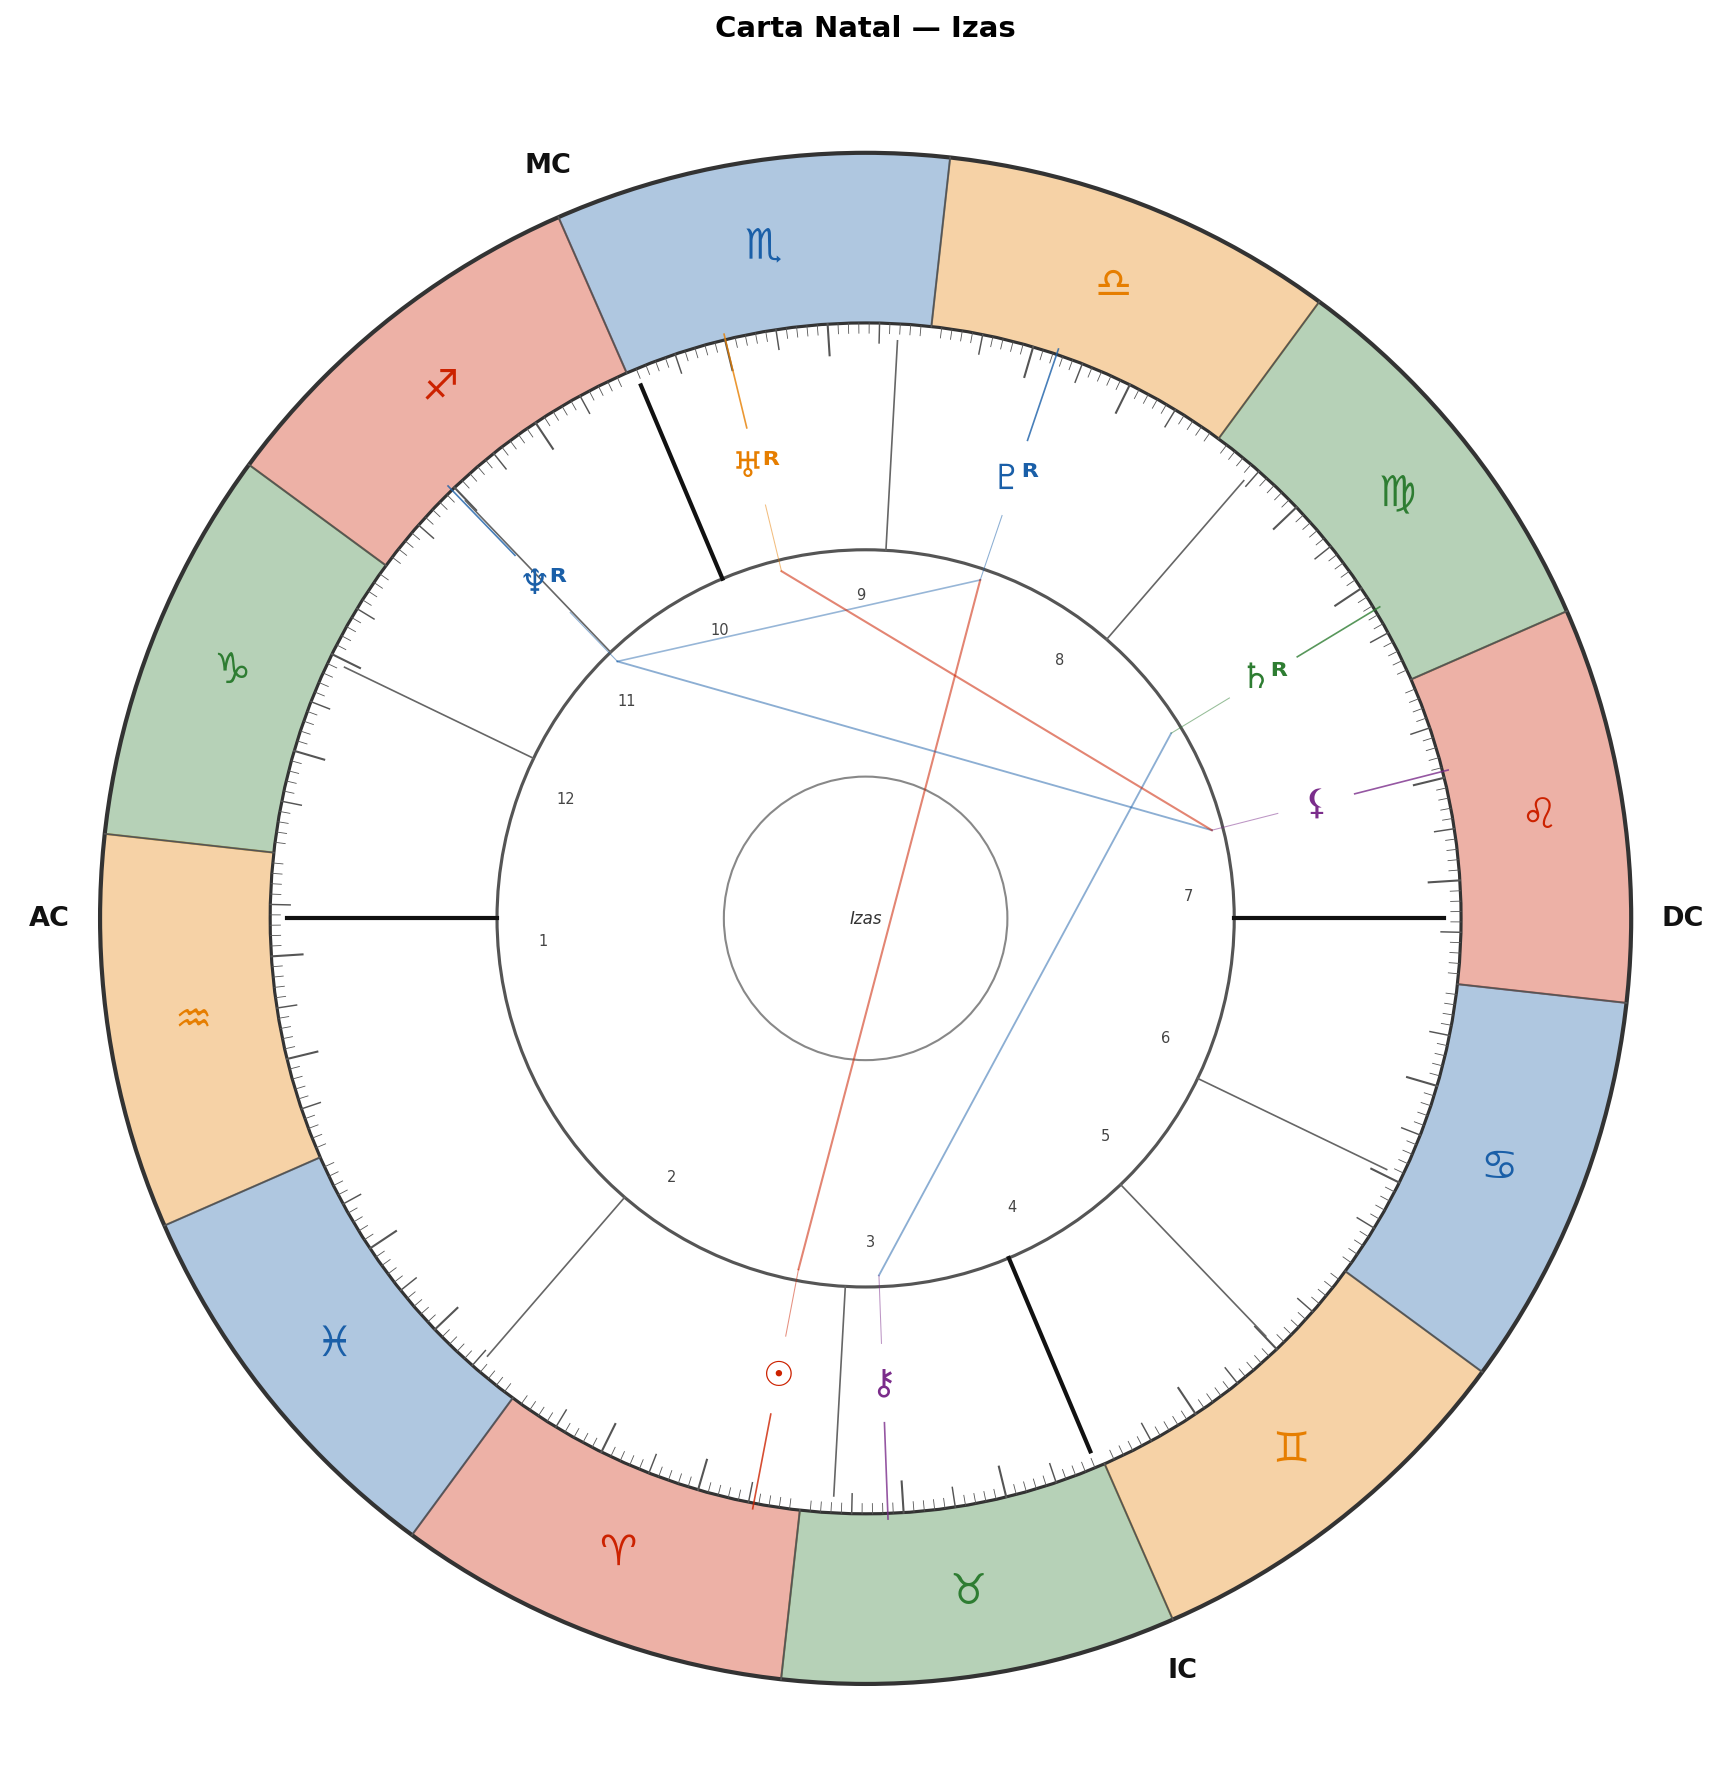
\includegraphics[width=0.72\textwidth]{Izas_rueda.png}
\end{center}

\Needspace{3\baselineskip}

\section{Interpretación}

\begin{center}
{\small\itshape
Este documento no busca definirte. Se acerca a zonas donde pueden aparecer intensidad,\\
defensa, herida, vulnerabilidad, deseo, retiro o dificultad para poner en palabras lo que ocurre.
}
\end{center}

\vspace{0.8cm}

\Needspace{10\baselineskip}
\vspace{0.4cm}

\subsection{1. Marco general}

Este documento entra en zonas de la carta que suelen vivirse con más intensidad, más defensa o más dificultad para nombrar. No describe una identidad fija ni una condena personal. Se acerca a lugares donde pueden aparecer miedo, control, vergüenza, deseo, aislamiento, dependencia, heridas antiguas o reacciones difíciles de comprender desde fuera.

Plutón en Libra, Casa 8: muestra dónde puedes vivir procesos intensos de transformación, pérdida de control, apego, defensa o profundidad emocional.
Quirón en Tauro, Casa 3: muestra una zona especialmente sensible, donde puede haber herida, inseguridad, vergüenza o necesidad de protección.
Lilith en Leo, Casa 7: muestra una parte de ti menos domesticable, más instintiva, que puede reaccionar con fuerza cuando se siente atrapada, reducida o invadida.

La Casa 8 en Virgo habla de cómo atraviesas la vulnerabilidad, la intimidad, la pérdida, la confianza y los vínculos que remueven profundamente.
La Casa 12 en Capricornio habla de cómo vives el retiro, la sensibilidad, el agotamiento emocional, lo inconsciente y aquello que cuesta poner en palabras.

Aspectos principales observados en este bloque: Plutón–Neptuno en sextil (orbe 2.71°), Plutón–Sol en oposición (orbe 7.88°), Quirón–Saturno en trígono (orbe 0.92°), Lilith–Neptuno en trígono (orbe 0.28°), Lilith–Urano en cuadratura (orbe 0.67°).

\Needspace{10\baselineskip}
\vspace{0.4cm}

\subsection{2. Plutón — Intensidad, control y transformación}

\Needspace{6\baselineskip}
\subsubsection*{Plutón en Libra — Casa 8 (retrógrado)}

Plutón en Libra muestra una intensidad profunda ligada al vínculo, el deseo, la dependencia, la comparación y el miedo al conflicto. Las relaciones pueden tocar zonas muy hondas de ti, especialmente cuando aparece la posibilidad de pérdida, rechazo o desequilibrio.

La sombra puede aparecer como complacencia, manipulación sutil, dependencia afectiva o necesidad de controlar la armonía para no sentir amenaza. A veces puedes ceder demasiado y luego resentirte por dentro.

La transformación pasa por mirar qué parte de ti negocia su verdad para no perder vínculo. Tu poder crece cuando puedes amar, elegir y relacionarte sin abandonar tu centro.

Plutón en casa 8 intensifica profundamente los temas de vulnerabilidad, intimidad, pérdida, deseo, control y transformación emocional. Sueles vivir ciertos procesos internos con mucha profundidad, incluso cuando desde fuera no se percibe.

Puede haber miedo a la traición, dificultad para confiar del todo o necesidad de mantener cierto control emocional para no sentirte expueste. A veces lo que más deseas también es lo que más miedo te da perder.

La transformación pasa por permitir cercanía sin vivir cada vínculo como un riesgo de destrucción. Tu profundidad deja de ser sufrimiento cuando no necesitas defenderla constantemente.

Plutón está retrógrado. La intensidad tiende a dirigirse primero hacia dentro. Puede haber procesos profundos que no se ven claramente desde fuera, pero que por dentro acumulan mucha fuerza. A veces tardas en mostrar lo que está ocurriendo, aunque internamente algo ya esté transformándose.

Plutón–Neptuno en sextil (orbe 2.71°).
Plutón en aspecto con Neptuno intensifica la sensibilidad, la percepción profunda y la relación con lo invisible o difícil de explicar. Puede haber mucha permeabilidad emocional, intuición o dificultad para distinguir entre deseo, miedo y fantasía.

A veces necesitas poner límites claros a lo que absorbes o idealizas.

El sextil abre una posibilidad de aprendizaje consciente. Puede no activarse solo, pero cuando le prestas atención permite trabajar esta combinación de una forma más manejable.

El orbe es relativamente cercano, así que esta combinación puede sentirse de forma bastante reconocible.

Plutón–Sol en oposición (orbe 7.88°).
Plutón en aspecto con el Sol toca directamente la identidad, la voluntad y la manera en que ocupas tu lugar. Puede haber intensidad en torno al poder personal, miedo a perder control o necesidad de transformarte profundamente a lo largo de la vida.

A veces puedes vivir ciertas etapas como crisis de identidad, momentos en los que una versión de ti deja de poder sostenerse.

La oposición suele vivirse como polaridad. A veces una parte de ti tira hacia un extremo y otra parte aparece reflejada en vínculos, conflictos o situaciones externas.

Aunque el orbe es más amplio, el aspecto puede seguir apareciendo como un matiz importante dentro de la carta.

\Needspace{10\baselineskip}
\vspace{0.4cm}

\subsection{3. Quirón — Herida, sensibilidad y protección}

\Needspace{6\baselineskip}
\subsubsection*{Quirón en Tauro — Casa 3}

Quirón en Tauro suele mostrar sensibilidad en torno al valor personal, la seguridad y la sensación de merecer estabilidad o bienestar. Puede haber miedo profundo a no tener suficiente o perder aquello que te sostiene.

A veces intentas construir seguridad desde el control, la acumulación o la autosuficiencia extrema. También puede costarte relajarte realmente en el cuerpo si dentro hay sensación constante de amenaza o carencia.

El aprendizaje pasa por descubrir que tu valor no depende únicamente de lo que produces, sostienes o consigues conservar.

Quirón en casa 3 suele mostrar sensibilidad respecto a la palabra, la comunicación y la forma de expresar lo que piensas. Puede haber miedo a decir algo incorrecto, a que no te entiendan o a sentir que tu voz no tiene suficiente peso.

A veces observas demasiado cómo hablas, explicas o respondes. También puede aparecer inseguridad intelectual o dificultad para confiar plenamente en tu propia percepción.

El aprendizaje pasa por permitir que tu voz exista sin exigirle perfección constante.

Quirón–Saturno en trígono (orbe 0.92°).
Quirón en aspecto con Saturno toca la exigencia, la responsabilidad y el miedo a fallar. Puede haber sensación de tener que demostrar mucho, sostener demasiado o no permitirte mostrar fragilidad.

A veces la herida se esconde detrás de una gran capacidad de aguante.

El trígono facilita que esta combinación fluya con más naturalidad. No elimina la profundidad del aspecto, pero puede hacer que encuentres recursos internos con mayor facilidad.

Este aspecto es muy cerrado, por lo que suele sentirse con bastante fuerza. No aparece como algo lejano o secundario, sino como una dinámica que puede activarse con claridad en momentos importantes.

\Needspace{10\baselineskip}
\vspace{0.4cm}

\subsection{4. Lilith — Lo no domesticado}

\Needspace{6\baselineskip}
\subsubsection*{Lilith en Leo — Casa 7}

Lilith en Leo muestra una parte de ti que necesita expresarse de forma auténtica y rechaza profundamente sentir que te anulan o invisibilizan. Puede haber mucha intensidad respecto al reconocimiento, la creatividad y el derecho a ocupar espacio.

A veces alternas entre mostrarte muchísimo y esconderte completamente por miedo a la exposición o al juicio. También puede aparecer necesidad de controlar cómo te perciben para proteger una vulnerabilidad muy profunda.

El aprendizaje pasa por permitirte brillar sin vivir la mirada ajena como una amenaza constante.

Lilith en casa 7 muestra intensidad en los vínculos y sensibilidad muy fuerte respecto a las dinámicas de dependencia, control o pérdida de libertad. Puede haber una parte de ti que desea mucha cercanía y al mismo tiempo teme profundamente quedar atrapade dentro de la relación.

A veces necesitas tomar distancia cuando el vínculo se vuelve demasiado invasivo o emocionalmente exigente. También puede aparecer atracción hacia relaciones intensas donde se activan dinámicas de poder difíciles de sostener.

El aprendizaje pasa por permitir vínculo sin sentir que necesitas desaparecer o defenderte constantemente.

Lilith–Neptuno en trígono (orbe 0.28°).
Lilith en aspecto con Neptuno intensifica la sensibilidad, el deseo de disolución y la dificultad para poner límites claros. Puede haber magnetismo, intuición y mucha permeabilidad emocional.

A veces cuesta distinguir entre entrega, idealización, deseo y huida.

El trígono facilita que esta combinación fluya con más naturalidad. No elimina la profundidad del aspecto, pero puede hacer que encuentres recursos internos con mayor facilidad.

Este aspecto es muy cerrado, por lo que suele sentirse con bastante fuerza. No aparece como algo lejano o secundario, sino como una dinámica que puede activarse con claridad en momentos importantes.

Lilith–Urano en cuadratura (orbe 0.67°).
Lilith en aspecto con Urano intensifica la diferencia, la independencia y el rechazo a encajar en lo esperado. Puede haber necesidad muy fuerte de espacio propio y de vivir según reglas internas.

A veces la cercanía se vuelve difícil cuando sientes que amenaza tu libertad.

La cuadratura suele generar tensión interna. Hay algo que necesita integrarse, pero normalmente no se vive de forma cómoda ni automática.

Este aspecto es muy cerrado, por lo que suele sentirse con bastante fuerza. No aparece como algo lejano o secundario, sino como una dinámica que puede activarse con claridad en momentos importantes.

\Needspace{10\baselineskip}
\vspace{0.4cm}

\subsection{5. Casa 8 — Intimidad, pérdida y vulnerabilidad}

\Needspace{6\baselineskip}
\subsubsection*{Casa 8 en Virgo}

La casa 8 en Virgo suele vivir los procesos emocionales profundos con mucha observación y necesidad de control. Puede haber dificultad para relajarte completamente en experiencias donde no puedes prever lo que ocurrirá.

A veces analizas demasiado lo que sientes o intentas ordenar emocionalmente algo que en realidad necesita ser atravesado. También puede aparecer hipervigilancia respecto a la vulnerabilidad propia o ajena.

El aprendizaje pasa por descubrir que no todo lo importante puede resolverse únicamente desde el control o la comprensión mental.

En tu carta, la Casa 8 contiene los siguientes planetas o puntos: Plutón.

Plutón en Casa 8.
Plutón en casa 8 intensifica profundamente todos los temas ligados a la vulnerabilidad, la intimidad y la transformación emocional. Las experiencias importantes suelen vivirse con mucha profundidad y rara vez desde la superficie.

Puede haber miedo fuerte a la pérdida, necesidad de control emocional o dificultad para confiar plenamente. También puede existir tendencia a vivir los vínculos desde intensidad extrema o hipervigilancia emocional.

El aprendizaje pasa por descubrir que profundidad no significa permanecer permanentemente en tensión o defensa.

\Needspace{10\baselineskip}
\vspace{0.4cm}

\subsection{6. Casa 12 — Retiro, sensibilidad y mundo interno}

\Needspace{6\baselineskip}
\subsubsection*{Casa 12 en Capricornio}

La casa 12 en Capricornio suele mostrar mucha contención emocional y dificultad para relajarte completamente. Puede haber sensación interna de tener que sostener demasiado incluso cuando estás agotade.

A veces te cuesta reconocer cansancio, necesidad o vulnerabilidad porque una parte de ti siente que no puede permitirse aflojar. También puede aparecer soledad emocional silenciosa detrás de una imagen fuerte o muy responsable.

El aprendizaje pasa por descubrir que descansar también es una forma de sostenerte.

En tu carta no hay planetas principales dentro de la Casa 12. Aun así, esta casa sigue hablando de cómo vives el retiro, la sensibilidad, el agotamiento emocional y aquello que cuesta poner en palabras.

\Needspace{10\baselineskip}
\vspace{0.4cm}

\subsection{7. Integración}

En conjunto, este bloque muestra una zona de lectura especialmente profunda de la carta. Plutón en Libra, Casa 8, señala dónde la intensidad puede obligarte a atravesar procesos de transformación real. Quirón en Tauro, Casa 3, muestra una sensibilidad que no siempre se deja tocar fácilmente. Lilith en Leo, Casa 7, señala una parte de ti que no acepta ser reducida, controlada o domesticada sin reaccionar.

La Casa 8 en Virgo describe cómo te acercas a la intimidad, la pérdida de control, la confianza y los vínculos que remueven. La Casa 12 en Capricornio muestra cómo se viven el cansancio profundo, el retiro, la sensibilidad y aquello que a veces permanece oculto incluso para ti.

Los aspectos tensos de este bloque indican zonas donde la intensidad, la herida o la reacción defensiva pueden aparecer con más fricción. No significan algo negativo en sí mismo, pero sí muestran lugares donde puede costarte integrar lo que sientes sin entrar en control, cierre o lucha interna.

Los aspectos fluidos muestran recursos internos para atravesar estas zonas con más naturalidad. No eliminan la intensidad, pero pueden facilitar comprensión, integración y mayor honestidad contigo.

La clave de este documento no es corregir estas zonas ni convertirlas en algo más amable de manera artificial. La clave es poder mirarlas sin rechazo, reconocer cuándo se activan y dejar de vivirlas únicamente desde la defensa, el silencio o el control.

\Needspace{10\baselineskip}
\vspace{0.4cm}

\subsection{8. Orientación}

\Needspace{6\baselineskip}
\subsubsection*{Cómo reconocer que esta zona está activa}
Puedes reconocer que este bloque está activo cuando una situación toca una zona desproporcionadamente sensible: miedo a perder el control, dificultad para confiar, necesidad de desaparecer, vergüenza, rabia contenida, deseo intenso, cierre emocional o sensación de amenaza interna.

Plutón en Casa 8 suele activarse cuando algo te obliga a mirar una intensidad que no puedes resolver solo desde la voluntad. Quirón en Casa 3 suele activarse cuando una experiencia toca una herida antigua o una sensación de insuficiencia. Lilith en Casa 7 suele activarse cuando sientes invasión, reducción, control o pérdida de libertad interna.

\Needspace{6\baselineskip}
\subsubsection*{Casa 8}
La Casa 8 en Virgo se activa especialmente en vínculos intensos, procesos de intimidad, pérdidas, dependencias, secretos, duelos o experiencias donde aparece vulnerabilidad real. Cuando esta zona se mueve, puedes sentir que algo dentro de ti necesita protegerse antes incluso de entender exactamente qué está ocurriendo.

\Needspace{6\baselineskip}
\subsubsection*{Casa 12}
La Casa 12 en Capricornio se activa especialmente en momentos de cansancio profundo, retiro, saturación emocional, confusión interna o necesidad de silencio. Cuando esta zona se mueve, puede costarte explicar lo que te pasa, pero eso no significa que no esté ocurriendo algo importante.

\Needspace{6\baselineskip}
\subsubsection*{Cuando no se reconoce}
Cuando estas zonas no se reconocen, es fácil vivirlas como problemas aislados: una relación que duele, una reacción excesiva, una etapa de agotamiento, una obsesión, una necesidad de control o una retirada que no sabes explicar.

Pero muchas veces no se trata solo de lo que ocurre fuera. Algo interno ha sido tocado y necesita ser mirado con más honestidad.

\Needspace{6\baselineskip}
\subsubsection*{Una forma más cuidadosa de mirarlo}
La orientación no es forzarte a abrir lo que todavía necesita protección. Tampoco se trata de justificar cualquier reacción porque venga de una herida. Se trata de reconocer con más precisión qué se activa, qué estás defendiendo y qué parte de ti necesita tiempo, verdad y cuidado.

\vspace{1cm}
\begin{center}
{\small\itshape\color{grisai}
La astrología se usa aquí como lenguaje simbólico de observación, no como definición cerrada de la persona.\
Este documento no sustituye ningún proceso terapéutico ni constituye un diagnóstico.
}
\end{center}

\end{document}
